\chapter{Unidad 4. Planificación del Procesador}

La planificación del procesador es una función crítica de los sistemas operativos que se encarga de gestionar cómo y cuándo los procesos reciben tiempo de CPU. Esta gestión es esencial para asegurar que todos los procesos en el sistema tengan un acceso justo y eficiente a los recursos del procesador.

\section{Niveles}
En un sistema operativo, la planificación del procesador se organiza en tres niveles principales, cada uno con un papel importante en la gestión eficiente de los recursos del sistema. Estos niveles determinan cómo y cuándo los procesos reciben acceso a la CPU.

\subsection{Planificación a largo plazo (Planificador de trabajos)}

\textbf{Función: }Este nivel de planificación se encarga de decidir qué procesos se deben admitir en el sistema. El planificador de trabajos controla la entrada de procesos nuevos en el sistema, determinando qué procesos deben ser cargados en la memoria principal para su ejecución.

En los sistemas modernos, la planificación a largo plazo es menos común, ya que los sistemas suelen tener la capacidad de manejar múltiples procesos sin necesidad de una planificación estricta a largo plazo. Sin embargo, sigue siendo relevante en sistemas con recursos limitados o en sistemas de procesamiento por lotes, donde se debe controlar la carga de trabajo.

\subsection{Planificación a Medio Plazo (Planificador de Swapping)}
\textbf{Función: }Este nivel de planificación gestiona la memoria y decide qué procesos deben ser movidos entre la memoria principal y la memoria secundaria (swap). El planificador a medio plazo es responsable de optimizar el uso de la memoria, asegurando que los procesos que necesitan más recursos estén en la memoria principal y los que están inactivos sean movidos al disco.

En los sistemas modernos, la planificación a medio plazo es crucial en la gestión de la memoria virtual. Aunque el término \textit{"swapping"} ha evolucionado, el concepto subyacente de manejar la memoria de manera eficiente sigue siendo esencial, especialmente en sistemas con un gran número de procesos activos.



\subsection{Planificación a Corto Plazo (Planificador del Procesador)}

\textbf{Función:} Este es el nivel de planificación más crítico y se encarga de decidir qué proceso en la cola de preparados debe ser ejecutado a continuación. El planificador a corto plazo realiza la conmutación de contexto y asegura que la CPU esté siempre ocupada ejecutando procesos. Lleva a cabo las funciones de la multiprogramación, estando siempre residente en memoria y ejecutándose con mucha frecuencia; estos procesos son de ejecución rápida.

\section{Objetivos}

Las políticas de planificación tienen como objetivo garantizar un uso eficiente y equitativo del procesador, además de optimizar el rendimiento general del sistema operativo. A continuación, se describen los principales objetivos que intentan cubrir estas políticas:

\subsection{Justicia}
La política de planificación debe ser justa, asegurando que todos los procesos tengan oportunidades equitativas de acceso a los recursos del sistema. Ningún proceso debe ser favorecido en detrimento de otro.

\textbf{Ejemplo:} En un sistema de tiempo compartido, todos los usuarios deben tener la misma oportunidad de acceder a la CPU sin que unos procesos monopolizen el tiempo de ejecución.

\subsection{Máxima Capacidad de Ejecución}
El objetivo es maximizar la capacidad de ejecución de la CPU, es decir, mantener el procesador ocupado el mayor tiempo posible con la menor cantidad de interrupciones. Esto se logra reduciendo el número de cambios de contexto, lo que permite que los trabajos se completen lo más rápidamente posible.

\textbf{Ejemplo:} Un algoritmo de planificación que minimiza los cambios de proceso permitirá que los trabajos se ejecuten con mayor fluidez, reduciendo el tiempo total de espera.

\subsection{Máximo Número de Usuarios Interactivos}
En sistemas de tiempo compartido, se busca que el mayor número posible de usuarios interactivos pueda trabajar simultáneamente. Esto mejora la experiencia de uso y la eficiencia en entornos multiusuario.

\textbf{Ejemplo:} En un sistema de servidores, es esencial que múltiples usuarios puedan acceder a sus aplicaciones o recursos al mismo tiempo sin que la velocidad o la respuesta se vean afectadas significativamente.

\subsection{Predecibilidad}
La política de planificación debe ser predecible, permitiendo saber cómo se ejecutarán los procesos en todo momento. Esto implica que el comportamiento del sistema sea consistente y que los procesos se ejecuten de acuerdo a las reglas establecidas.

\textbf{Ejemplo:} En un sistema crítico, como el de control de tráfico aéreo, es importante que las aplicaciones respondan de manera predecible, asegurando que las tareas críticas siempre se ejecuten en el tiempo adecuado.

\subsection{Minimización de la Sobrecarga}
El objetivo es reducir la sobrecarga del sistema. Esto incluye minimizar los cambios de contexto y las operaciones innecesarias que ralentizan el rendimiento del sistema. Cuanto menor sea la sobrecarga, mayor será la velocidad de procesamiento general del sistema.



\subsection{Equilibrio en el Uso de Recursos}
Es esencial que los recursos del sistema (CPU, memoria, dispositivos de entrada/salida) se utilicen de manera equilibrada. Esto implica que los recursos estén ocupados de manera justa y eficiente para obtener un buen rendimiento general.

\textbf{Ejemplo:} Si un proceso está utilizando demasiados recursos de E/S, el sistema operativo puede reducir su acceso a la CPU para que otros procesos tengan la oportunidad de ejecutarse.

\subsection{Seguridad de las Prioridades}
Los procesos de mayor prioridad deben recibir más atención del procesador y ejecutarse más rápidamente que aquellos con menor prioridad. Esto asegura que los procesos críticos no se vean retrasados por procesos menos importantes.

\textbf{Ejemplo:} Un proceso del sistema que gestiona la seguridad debe tener prioridad sobre los procesos de los usuarios comunes, asegurando que se ejecute sin demoras.


\section{Criterios}

Los criterios que se deben tener en cuenta a la hora de elegir o diseñar un algoritmo de planificación son los siguientes:

\subsection{Tiempo de Respuesta}
Es la velocidad con que el ordenador da respuesta a una petición. Depende principalmente de la velocidad de los dispositivos de entrada/salida (E/S), la carga del sistema y el algoritmo de planificación empleado.

\subsection{Tiempo de Servicio}
Es el tiempo total que tarda en ejecutarse un proceso. Este incluye el tiempo de carga del programa en la memoria, el tiempo de espera en la cola de procesos preparados, el tiempo de ejecución en el procesador, y el tiempo consumido en operaciones de E/S.

\subsection{Tiempo de Ejecución}
Es idéntico al tiempo de servicio, pero excluye el tiempo de espera en la cola de procesos preparados. Es el tiempo que necesitaría el proceso para completarse si fuera el único en ejecución en el sistema.

\subsection{Tiempo de Procesador}
Es el tiempo que un proceso está utilizando activamente el procesador, sin contar los periodos en los que se encuentra bloqueado, por ejemplo, debido a operaciones de E/S.

\subsection{Tiempo de Espera}
Es el tiempo en que los procesos están activos pero sin ser ejecutados, es decir, el tiempo que pasan en las colas de espera, como la cola de procesos preparados.

\subsection{Eficiencia}
La eficiencia se refiere a la utilización del procesador, el recurso más valioso en un sistema. El objetivo es que el procesador esté ocupado el mayor tiempo posible para maximizar el rendimiento, con el menor tiempo de inactividad.

\subsection{Rendimiento}
Es el número de trabajos o procesos completados por unidad de tiempo. El rendimiento óptimo se alcanza cuando el sistema es capaz de gestionar el mayor número de tareas posible en un periodo de tiempo, dependiendo del algoritmo de planificación y la carga del sistema.

\section{Medidas en la Planificación de Procesos}

Para evaluar cómo se comportan las diferentes políticas de planificación del procesador, utilizamos una serie de medidas que nos permiten analizar el rendimiento del sistema y cómo se gestionan los procesos.

\subsection{Tiempo de Servicio (T)}
El \textbf{tiempo de servicio} es el tiempo total que un proceso tarda en ejecutarse completamente desde el momento en que se da la orden de ejecución hasta que termina.

\textbf{Fórmula:} 
\[
T = t_{\text{fin}} - t_{\text{inicio}}
\]

Donde:
\begin{itemize}
	\item \( t_{\text{inicio}} \) es el momento en que el proceso comienza su ejecución.
	\item \( t_{\text{fin}} \) es el momento en que el proceso termina.
\end{itemize}

\textbf{Ejemplo:} Si un proceso comienza a ejecutarse a las 3:00 p.m. y termina a las 3:10 p.m., el tiempo de servicio sería 10 minutos.

\subsection{Tiempo de Espera (E)}
El \textbf{tiempo de espera} es el tiempo que un proceso pasa en cola, esperando a ser ejecutado. Es la diferencia entre el tiempo total del proceso y el tiempo en que realmente está usando la CPU.

\textbf{Fórmula:}
\[
E = T - t
\]

Donde:
\begin{itemize}
	\item \( T \) es el tiempo de servicio.
	\item \( t \) es el tiempo que el proceso pasa en ejecución.
\end{itemize}

\textbf{Ejemplo:} Si el tiempo total de servicio es 10 minutos, pero el proceso solo estuvo ejecutándose durante 7 minutos, el tiempo de espera sería 3 minutos.

\newpage

\subsection{Índice de Servicio (I)}
El \textbf{índice de servicio} nos indica qué tanto tiempo un proceso estuvo ejecutándose en comparación con su tiempo total en el sistema.

\textbf{Fórmula:}
\[
I = \frac{t}{T}
\]

Donde:
\begin{itemize}
	\item \( t \) es el tiempo de ejecución del proceso.
	\item \( T \) es el tiempo de servicio total.
\end{itemize}


\textbf{Interpretación:}
\begin{itemize}
	\item Un valor de \( I \) cercano a \textit{1} indica que el proceso estuvo ejecutándose la mayor parte del tiempo que estuvo en el sistema, es decir, tuvo poco tiempo de espera.
	\item Un valor de \( I \) cercano a \textit{0} indica que el proceso pasó una parte significativa de su tiempo \textbf{esperando} en cola antes de ser ejecutado.
\end{itemize}

\textbf{Ejemplo:}

Supongamos que un proceso tiene:
\begin{itemize}
	\item Tiempo de servicio total \( T = 10 \) minutos.
	\item Tiempo de ejecución \( t = 4 \) minutos.
\end{itemize}

Entonces, el Índice de Servicio sería:
\[
I = \frac{t}{T} = \frac{4 \text{ minutos}}{10 \text{ minutos}} = 0.4
\]
Esto significa que el proceso estuvo ejecutándose el **40\%** del tiempo total que estuvo en el sistema y esperando el **60\%** restante.




\subsection{Tiempo del Núcleo}
Es el tiempo que consume el núcleo del sistema operativo para tomar decisiones sobre la planificación del procesador. Este tiempo incluye los cambios de contexto, es decir, cuando el sistema guarda el estado de un proceso y carga el estado de otro para ejecutar.

\subsection{Tiempo de Inactividad (Idle)}
Es el tiempo en que la CPU no tiene ningún trabajo productivo que realizar. Esto ocurre cuando no hay procesos listos para ejecutarse, es decir, cuando la cola de procesos preparados está vacía.

\textbf{Ejemplo:} Si la computadora está encendida pero no tiene ninguna tarea que procesar, el tiempo de inactividad aumenta. Aunque el sistema sigue funcionando, la CPU está ``esperando'' por nuevas tareas.



\section{Algoritmos de planificación}

Antes de detallar los algoritmos de planificación, es importante entender las dos políticas principales que guían la planificación de los procesos:

\begin{enumerate}
	\item \textbf{Política Apropiativa:}
	En esta política, un proceso puede ser interrumpido mientras está ejecutándose y ser reemplazado por otro proceso. Esto ocurre con frecuencia cuando llega un proceso de mayor prioridad o cuando se cumple el límite de tiempo asignado al proceso en la CPU.
		
	\textbf{Ventaja:} Permite una respuesta más rápida a procesos críticos o de mayor prioridad.
	
	\textbf{Desventaja:} Genera más cambios de contexto, lo que puede aumentar la sobrecarga del sistema.
	\item \textbf{Política No Apropiativa:}
	En este caso, una vez que un proceso empieza a ejecutarse, no es interrumpido hasta que se completa. No importa si llegan procesos de mayor prioridad o más cortos durante su ejecución.
	
	\textbf{Ventaja:} Menos cambios de contexto, lo que reduce la sobrecarga del sistema.
	
	\textbf{Desventaja:} Puede hacer que procesos críticos o urgentes tengan que esperar más tiempo.
	
\end{enumerate}





\subsection{Algoritmo FCFS (First Come First Served)} El algoritmo FCFS (First Come First Served), o Primero en llegar, primero en ser atendido, es el algoritmo de planificación más simple. Los procesos son gestionados en una cola única de procesos listos, y se ejecutan en el orden en que llegan. El primer proceso en entrar a la cola será el primero en recibir el tiempo de CPU, y no será interrumpido hasta que termine su ejecución.

\textbf{Características del FCFS:}
\begin{itemize} \item Política no apropiativa: Una vez que el proceso comienza a ejecutarse, no se interrumpe hasta que se completa. \item Los procesos se ejecutan por orden de llegada: El primer proceso en llegar es el primero en ser atendido. \item Todos los procesos esperan en una sola cola: Los procesos en la cola deben esperar su turno hasta que el CPU esté libre. \end{itemize}

\begin{figure}[H] \centering 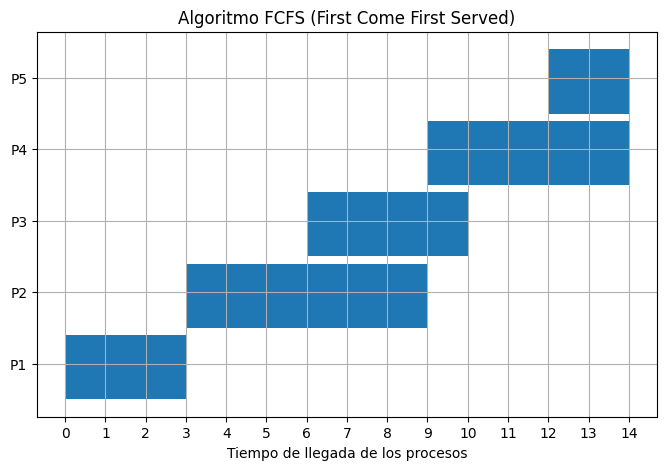
\includegraphics[width=0.8\linewidth]{Imagenes/Fcfs_tiempo.png} \caption{Se puede observar la llegada de los procesos y su tiempo de ejecución.} \end{figure}

\subsubsection{Ejecución según FCFS} Como ya se ha descrito, la ejecución de procesos mediante el algoritmo FCFS se realiza a partir de una sola cola, en orden de llegada. La llegada de un nuevo proceso lo ubicará automáticamente al final de la cola, lo que puede incrementar los tiempos de espera de los procesos más cortos que llegan después de uno largo.

\begin{figure}[H] \centering 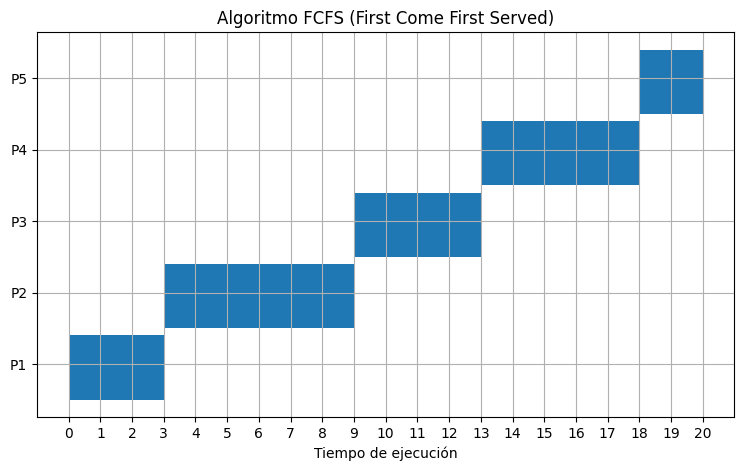
\includegraphics[width=0.8\linewidth]{Imagenes/fcfs_ejecucion.png} 
	\caption{Cola de procesos en ejecución para el algoritmo FCFS.} 
\end{figure}


\begin{itemize}
	\item P1 llega en el tiempo 0 y se ejecuta por 3 unidades de tiempo (de 0 a 3).
	\item 	P2 llega en el tiempo 3 y se ejecuta por 6 unidades de tiempo (de 3 a 9).
	\item 	P3 llega en el tiempo 6, pero espera hasta que P2 termine, y luego se ejecuta por 4 unidades de tiempo (de 9 a 13).
	\item 	
	P4 llega en el tiempo 9, pero espera hasta que P3 termine, y se ejecuta por 5 unidades de tiempo (de 13 a 18).
	\item P5 llega en el tiempo 12 y se ejecuta al final por 2 unidades de tiempo (de 18 a 20).
	
	
\end{itemize}


\subsection{Algoritmo Round Robin (RR)}

El algoritmo Round Robin (RR) es uno de los algoritmos de planificación más utilizados, especialmente en sistemas de tiempo compartido. En este algoritmo, cada proceso recibe una porción de tiempo fija, llamada cuanto de tiempo o quantum, para ejecutarse en la CPU. Si el proceso no se completa en ese tiempo, se coloca al final de la cola y se le asigna otro cuanto de tiempo en su siguiente turno. Este proceso se repite hasta que el proceso termine su ejecución.

\textbf{Características del Round Robin (RR):}
	\begin{itemize} 
		\item Política apropiativa: Si el proceso no termina dentro de su cuanto de tiempo, se interrumpe y se coloca al final de la cola de procesos listos. 
		\item Cuanto de tiempo fijo: Todos los procesos reciben la misma cantidad de tiempo para ejecutarse en cada ciclo, lo que asegura que todos los procesos reciban una oportunidad justa para usar la CPU. 
		\item Cola circular de procesos listos: Los procesos se ejecutan en orden y, si no terminan, se colocan nuevamente en la cola para su próxima oportunidad.
	\end{itemize}

\subsubsection{Ejecución según Round Robin}
	
El Round Robin es ideal para sistemas interactivos donde se necesita que todos los procesos reciban un tiempo de CPU de manera equitativa. El tamaño del cuanto de tiempo es crucial: si es muy pequeño, el sistema pasa mucho tiempo en cambios de contexto; si es muy grande, el algoritmo se comporta como FCFS.
\begin{figure}[H] \centering 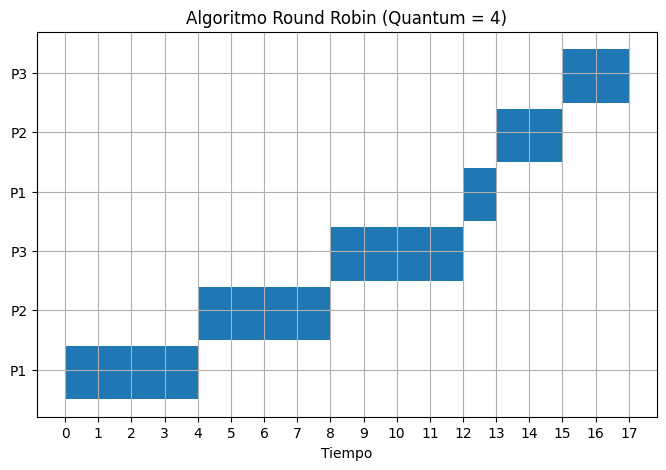
\includegraphics[width=0.8\linewidth]{Imagenes/rr_ejecucion.png} 
	\caption{Algoritmo RR en ejecución.} 
\end{figure}

\textbf{Ejemplo con \textit{quantum} de 4 unidades:}
\begin{itemize}
	\item 
	P1 tiene un tamaño 5, llega en el tiempo 0 y se ejecuta por 4 unidades de tiempo (de 0 a 4). Luego, se coloca al final de la cola.
	\item 	P2 llega con tamaño 6 y se ejecuta por 4 unidades de tiempo (de 4 a 8).
	\item 	P3 llega con tamaño 6, y se ejecuta por 4 unidades de tiempo (de 8 a 12).
	\item 	
	P1 completa su ejecución (12 a 13).
	\item P2 vuelve a ejecutarse por 2 unidades de tiempo (de 13 a 15), completando su ejecución.
	\item P3 vuelve a ejecutarse por 2 unidades de tiempo (de 15 a 17), completando su ejecución.
	
\end{itemize}

\subsection{Algoritmo SJN (Shortest Job Next)}

El algoritmo Shortest Job Next (SJN), también conocido como Shortest Process Next (SPN), selecciona el proceso con la menor duración estimada de ejecución para ser ejecutado a continuación. Es un algoritmo eficiente en términos de minimizar el tiempo promedio de espera en sistemas donde se conoce la duración de los procesos antes de que comiencen.

\textbf{Características del SJN:}
\begin{itemize} 
	\item Política no apropiativa: Una vez que el proceso con la menor duración es seleccionado, se ejecuta hasta su finalización sin interrupciones. 
	\item Minimización del tiempo promedio de espera: Como se priorizan los procesos más cortos, se optimiza el tiempo promedio de espera de todos los procesos en el sistema. \item Requiere conocimiento previo: El algoritmo necesita conocer la duración de cada proceso antes de su ejecución, lo cual puede no ser factible en algunos sistemas. \item Problema del ``hambre'': Los procesos largos pueden quedar esperando indefinidamente si continuamente llegan procesos más cortos, lo que se conoce como el problema del ``hambre'' o starvation. 
\end{itemize}

\subsubsection{Ejecución según SJN}

El algoritmo SJN selecciona siempre el proceso que tiene la menor duración para ejecutarse primero. Si varios procesos tienen la misma duración, se ejecuta el que llegó primero, similar a FCFS en este caso.

\textbf{Ejemplo:}
Supongamos que tenemos los siguientes procesos, cada uno con su tiempo de llegada y duración estimada de ejecución:

\begin{figure}[H] \centering 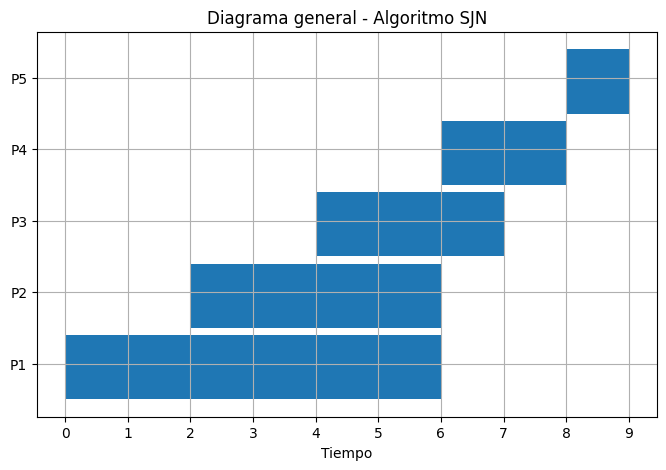
\includegraphics[width=0.8\linewidth]{Imagenes/snj_esquema.png} 
	\caption{Cola de procesos en ejecución para el algoritmo SJN.} 
\end{figure}



\begin{itemize} 
	\item P1 llega en el tiempo 0 y tiene una duración de 6 unidades de tiempo. 
	\item P2 llega en el tiempo 2 y tiene una duración de 4 unidades de tiempo. 
	\item P3 llega en el tiempo 4 y tiene una duración de 3 unidades de tiempo. 
	\item P4 llega en el tiempo 6 y tiene una duración de 2 unidades de tiempo. 
	\item P5 llega en el tiempo 8 y tiene una duración de 1 unidad de tiempo. 
\end{itemize}
Entonces la ejecución se daría de la siguiente forma:
\begin{figure}[H] \centering 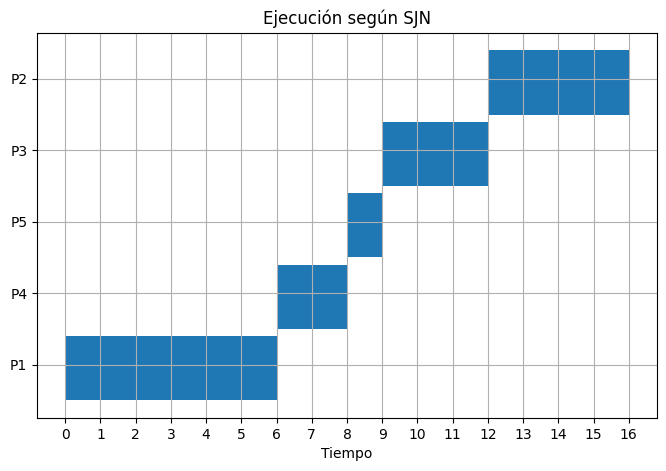
\includegraphics[width=0.8\linewidth]{Imagenes/sjn_ejecucion.png} 
	\caption{Ejecución de procesos para el algoritmo SJN.} 
\end{figure}
\begin{itemize} 
    \item P1 llega en el tiempo 0 y se ejecuta, pues en ese momento es el único proceso. 
    \item P4 llega en el tiempo 6 y se ejecuta a continuación, pues es el de menor duración. 
    \item P5 llega en el tiempo 8 y es el siguiente en ejecutarse. 
    \item P3 llega en el tiempo 4 y es el próximo en ejecución. 
    \item P2 llega en el tiempo 2 y es el último en ejecutarse. 
\end{itemize}



\subsection{Algoritmo SRT (Shortest Remaining Time)}

El algoritmo Shortest Remaining Time (SRT), también conocido como Shortest Remaining Time First (SRTF), es una variante del algoritmo SJN (Shortest Job Next), pero con la característica de que es un algoritmo apropiativo. Esto significa que un proceso en ejecución puede ser interrumpido si llega otro proceso con un tiempo de ejecución restante menor.

\textbf{Características del SRT:} 
\begin{itemize} 
    \item Política apropiativa: Si un proceso con menor tiempo de ejecución restante llega mientras otro proceso está en ejecución, el proceso actual es interrumpido y se le da prioridad al nuevo proceso. 
    \item Minimización del tiempo promedio de espera: Al igual que en SJN, los procesos más cortos tienen prioridad, lo que reduce el tiempo promedio de espera en el sistema. 
    \item Eficiente para tiempos dinámicos: A diferencia de SJN, donde es necesario conocer la duración total de los procesos antes de ejecutarse, SRT permite tomar decisiones a medida que nuevos procesos llegan al sistema. 
    \item Problema del "hambre": Los procesos largos pueden ser interrumpidos continuamente si nuevos procesos más cortos siguen llegando, lo que puede causar que un proceso largo nunca termine. 
\end{itemize}